\section{Regionale Entwicklung}

\subsection{Einflussfaktoren die zur Entstehung von Wirtschaftsräumen in Österreich beitragen}

\subsubsection{Urbanisierung}

Die zunehmende Urbanisierung ist ein wesentlicher Treiber für die Entstehung von Wirtschaftsräumen in Österreich. Großstädte wie Wien, Linz und Graz ziehen Unternehmen, Arbeitskräfte und Investitionen an und bieten eine Vielzahl von wirtschaftlichen Möglichkeiten. Durch die Nähe zu urbanen Zentren wird ein dichtes Netzwerk von wirtschaftlichen Aktivitäten gebildet und fördert die Bildung von Wirtschaftsräumen.

\subsubsection{Infrastruktur}

Eine gut ausgebaute Infrastruktur ist ebenfalls entscheidend für die Entwicklung und Bildung von Wirtschaftsräumen. Gut entwickelte Verkehrswege wie Autobahnen, Schienenverbindungen und Flughäfen erleichtern den Transport von Gütern und Personen und fördern die Mobilität innerhalb des Landes und über die Grenzen dieses hinaus.

\subsubsection{Bildungs- und Forschungseinrichtungen}

Die Präsenz von Bildungs- und Forschungseinrichtungen wie Universitäten, Fachhochschulen und Forschungsinstitute fördert die Bildung von Wirtschaftsräumen. Diese Institutionen dienen als Quelle für qualifizierte Arbeitskräfte, fördern Innovationen und unterstützen die Zusammenarbeit zwischen Bildung, Wissenschaft und Wirtschaft

\subsubsection{Clusterbildung}

Die Bildung von Branchenclustern, in denen Unternehmen aus zusammenarbeitenden Branchen räumlich konzentriert sind, ist ein weiterer Einflussfaktor. Durch die Nähe zueinander können Unternehmen von Synergieeffekten profitieren, wie beispielsweise gemeinsame Zulieferer, Fachkräftepools und Wissenstransfer. Dies förder die Wettbewerbsfähigkeit und trägt zur Entstehung von Wirtschaftsräumen bei.

\subsubsection{Regionale Förderpolitik}

Die gezielte Förderung bestimmter Regionen durch staatliche Maßnahmen kann ebenfalls zur Entstehung von Wirtschaftsräumen beitragen. Durch Investitionen in Infrastrukturprojekte, Bildungsinitiativen und Wirtschaftsförderung können strukturschwache Regionen gestärkt und neue wirtschaftliche Impulse gesetzt werden.

\subsubsection{Zusammenfassung}

Insgesamt sind diese Einflussfaktoren eng miteinander verbunden und tragen gemeinsam zur Entstehung und Entwicklung von Wirtschaftsräumen in Österreich bei. Sie formen das wirtschaftliche Gefüge des Landes und prägen die regionale Wirtschaftslandschaft.

\subsection{Wichtige Wirtschaftsräume Österreichs}

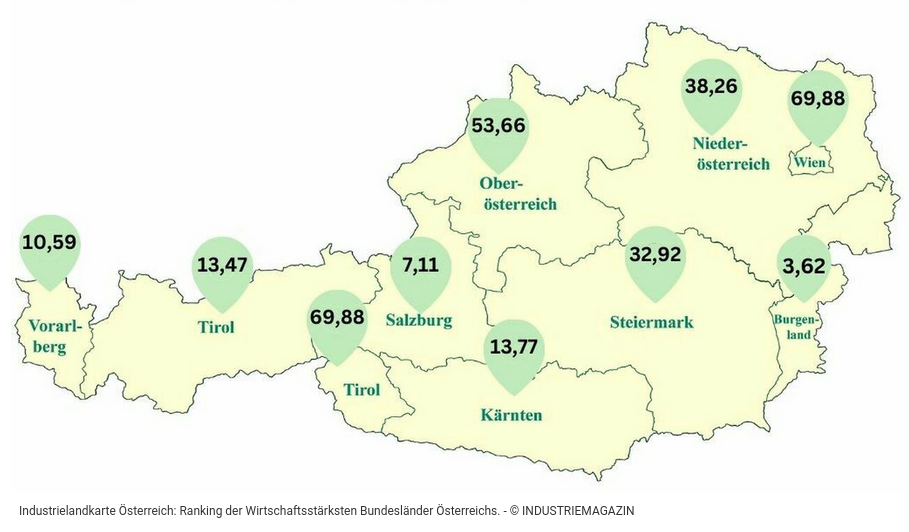
\includegraphics[scale=0.4]{Wirtschaftsstärke_Bundesländer.png}

Wie auf der Grafik zu sehen ist sind die Wirtschaftsstärksten Bundesländer Wien und Tirol, gefolgt von Ober- und Niederösterreich. Die Werte in der Grafik sind in Mrd. Euro angegeben und geben die österreichische Industrieproduktion wieder. In Wien sind Werke in denen Weltunternehmen, wie Bombardier oder Siemens, produzieren. Bei den zuvor genannten Unternehmen werden in Wien beispielsweise Straßenbahnen entwickelt und gebaut. Auch die Firma Rheinmetall baut in Wien ihre gepanzerten Lastkraftwagen, welche beim österreichischen Bundesheer, bei der deutschen Bundeswehr und bei der polnischen Armee im Einsatz sind. Weiters sind, wie zuvor genannt, ein gut ausgebautes Verkehrsnetz und Bildungsmöglichkeiten in Wien vorhanden, damit ein Wirtschaftsraum entstehen konnte und weiter bestehen kann. 

\subsection{Industriecluster in Österreich}

\subsubsection{Oberösterreich}

In Oberösterreich gibt es viele große und wichtige Cluster. Diese Cluster sind in den Branchen Automobilherstellung, IT, Kunststoff, Mechatronik, Medizintechnik, Umwelttechnik, Luft- und Raumfahrt und Möbel- und Holzbau.

\subsubsection{Niederösterreich}

In Niederösterreich gibt es zwar weniger Cluster, jedoch sind diese nicht weniger wichtiger als jene in Oberösterreich. In den Feldern Bau, Energie, Umwelt, Lebensmittel, Kunststoff und Mechatronik bestehen momentan im Bundesland Niederösterreich Industriecluster von Firmen, die zusammenarbeiten.   

\subsubsection{Tirol}

In Tirol ist die Clusterbildung am geringsten, es gibt nämlich nur 5 Cluster. Diese sind in den Sparten Erneuerbare Energie, IT, Life Sciences, Mechatronik und Wellness.

\subsubsection{andere Bundesländer}

In den anderen Bundesländern gibt es auch Cluster, diese sind aber entweder für sehr spezifische oder für nicht so relevante Bereiche zuständig.

\subsection{Wirtschaft in Österreich}

In der folgenden Grafik ist das BIP pro Kopf für die jeweiligen Bundesländer für das Jahr 2022 zu sehen. In dieser Statistik sind, nicht wie in der vorherigen Grafik, alle Sektoren und Einkünfte einbezogen und nicht nur aus dem Industriesektor.

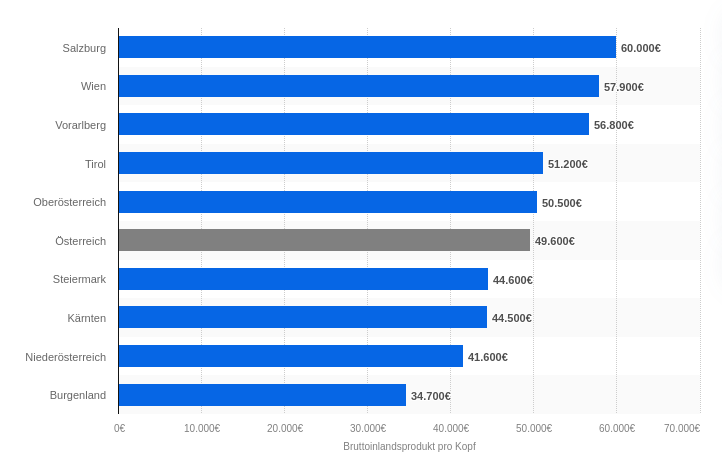
\includegraphics[scale=0.45]{BIP_Oesterreich.png}

In Salzburg und Wien ist vorallem der Tourismus für das Brutto Inlands Produkt fördernd, da in diesen Bundesländern viele Touristen aus dem In- und Ausland anreisen. Außerdem sind große Unternehmen in diesen Bundesländern angesiedelt, was den Wert weiter in die Höhe treibt.

\section{Herausforderungen und Chancen}

\subsection{Herausforderungen}

\subsubsection{Strukturwandel}

Die Globalisierung kann zu einem Strukturwandel in manchen Wirtschaftszweigen führen besonders in traditionellen Industrien wie Bergbau, Landwirtschaft und Fertigung. Regionen, welche mit stark von diesen betroffenen Branchen abhängig sind, stehen diese vor Herausforderungen sich an die neue wirtschaftliche Realität anzupassen und alternative Möglichkeiten für Arbeitsplätze zu schaffen.

\subsubsection{Abwanderung}

Die Globalisierung kann zu Abwanderungstendenzen, insbesondere von junger und hochqualifizierter Arbeitskräfte führen, die ins Ausland oder Ballungszentren ziehe, damit ihnen beruflich bessere Chancen bevor stehen. Solche Abwanderungen kann zu einem Brain Drain, also zu einem Wissensverlust im Land führen und die demografische Struktur bestimmter Regionen beeinflussen, was wiederum Herausforderungen für die lokale Wirtschaft und Gemeinschaften mit sich bringt.

\subsection{Chancen}

\subsubsection{Entwicklung in ländlichen und strukturschwachen Gebieten}

Die Globalisierung bietet auch Chancen für eine nachhaltige Entwicklung in ländlichen und strukturschwachen Gebieten. Durch den Zugang zu internationalen Märkten können lokale Unternehmen neue Absatzmärkte erschließen und ihre Wettbewerbsfähigkeit steigern. Gleichzeitig können modernen Technologien und digitale Plattformen es Unternehmen in ländlichen Gebieten ermöglichen remote zu arbeiten und ihre Produkte und Dienstleistungen global anzubieten.

\subsubsection{Innovationspotenzial}



\subsection{Strategien und Handlungsempfehlungen}

\subsubsection{Diversifizierung der Wirtschaft}

\subsubsection{Stärkung der regionalen Zusammenarbeit}

\subsubsection{Gezielte Investitionen in Infrastruktur und Bildung}